\section{Transiente Stabilität}
    \textit{Transiente Stabilität} bezieht sich auf die Fähigkeit der Synchronität eines zusammengeschalteten Stromnetzes, 
    nach einer Störung synchron zu bleiben. Sie hängt von der Fähigkeit ab, 
    das Gleichgewicht zwischen dem elektromagnetischen Drehmoment und dem mechanischen Drehmoment 
    jeder Synchronmaschine im System aufrechtzuerhalten bzw. wiederherzustellen.

\subsection{Mechanische zu Elektrischer Leistung}
    \begin{minipage}[t]{0.49\columnwidth}
        \centering \vspace{-0.7\baselineskip}
        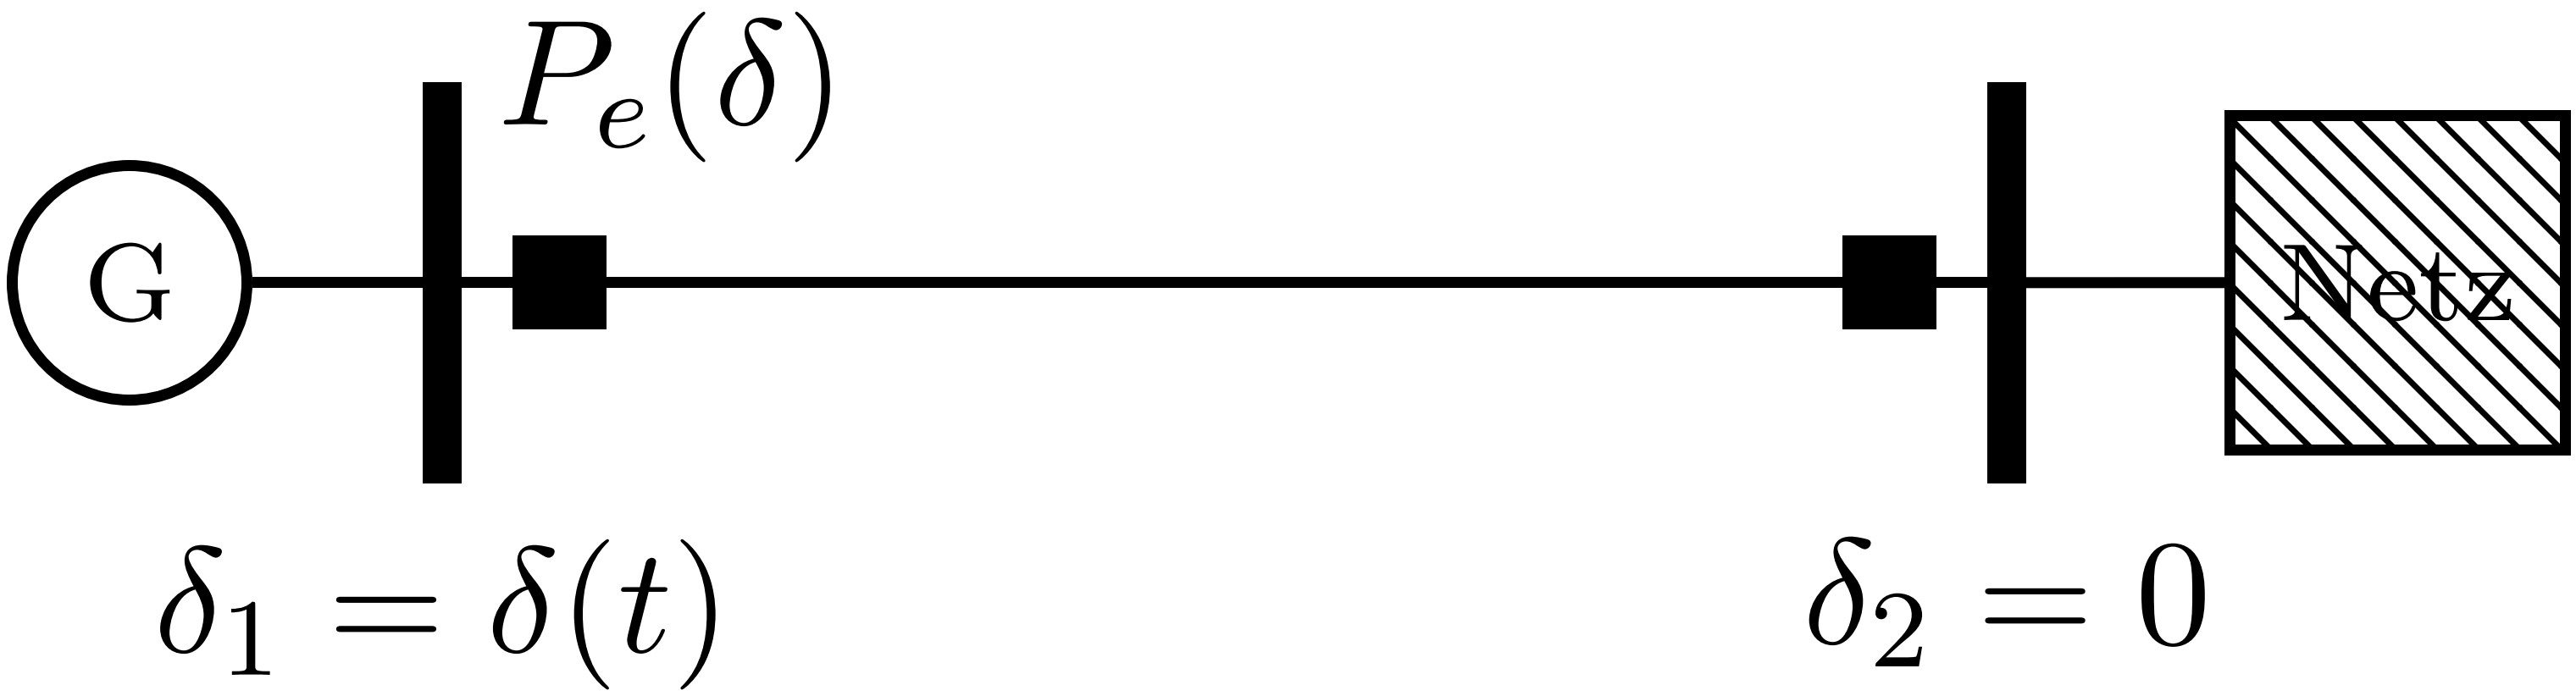
\includegraphics[width=0.95\linewidth]{images/Transiente_Stabilität.jpg}
    \end{minipage}%
    \hfill
    \begin{minipage}[t]{0.49\columnwidth}
        \centering \vspace{-0.7\baselineskip}
        $\boxed{\frac{d\omega}{dt} = \frac{P_m - P_e}{2H}}$
        $\quad$
        $\boxed{\frac{d\delta}{dt} = \omega}$
    \end{minipage}

    \vspace{0.1cm}

    Im stabilen Zustand gilt:  $P_m = P_e \; \Rightarrow \; \frac{d\omega}{dt} = 0$

\subsubsection{Fehlerfall, Lastabwurf, $P_e = 0$}
    \begin{minipage}[t]{0.49\columnwidth}
        \centering \vspace{-0.7\baselineskip}
        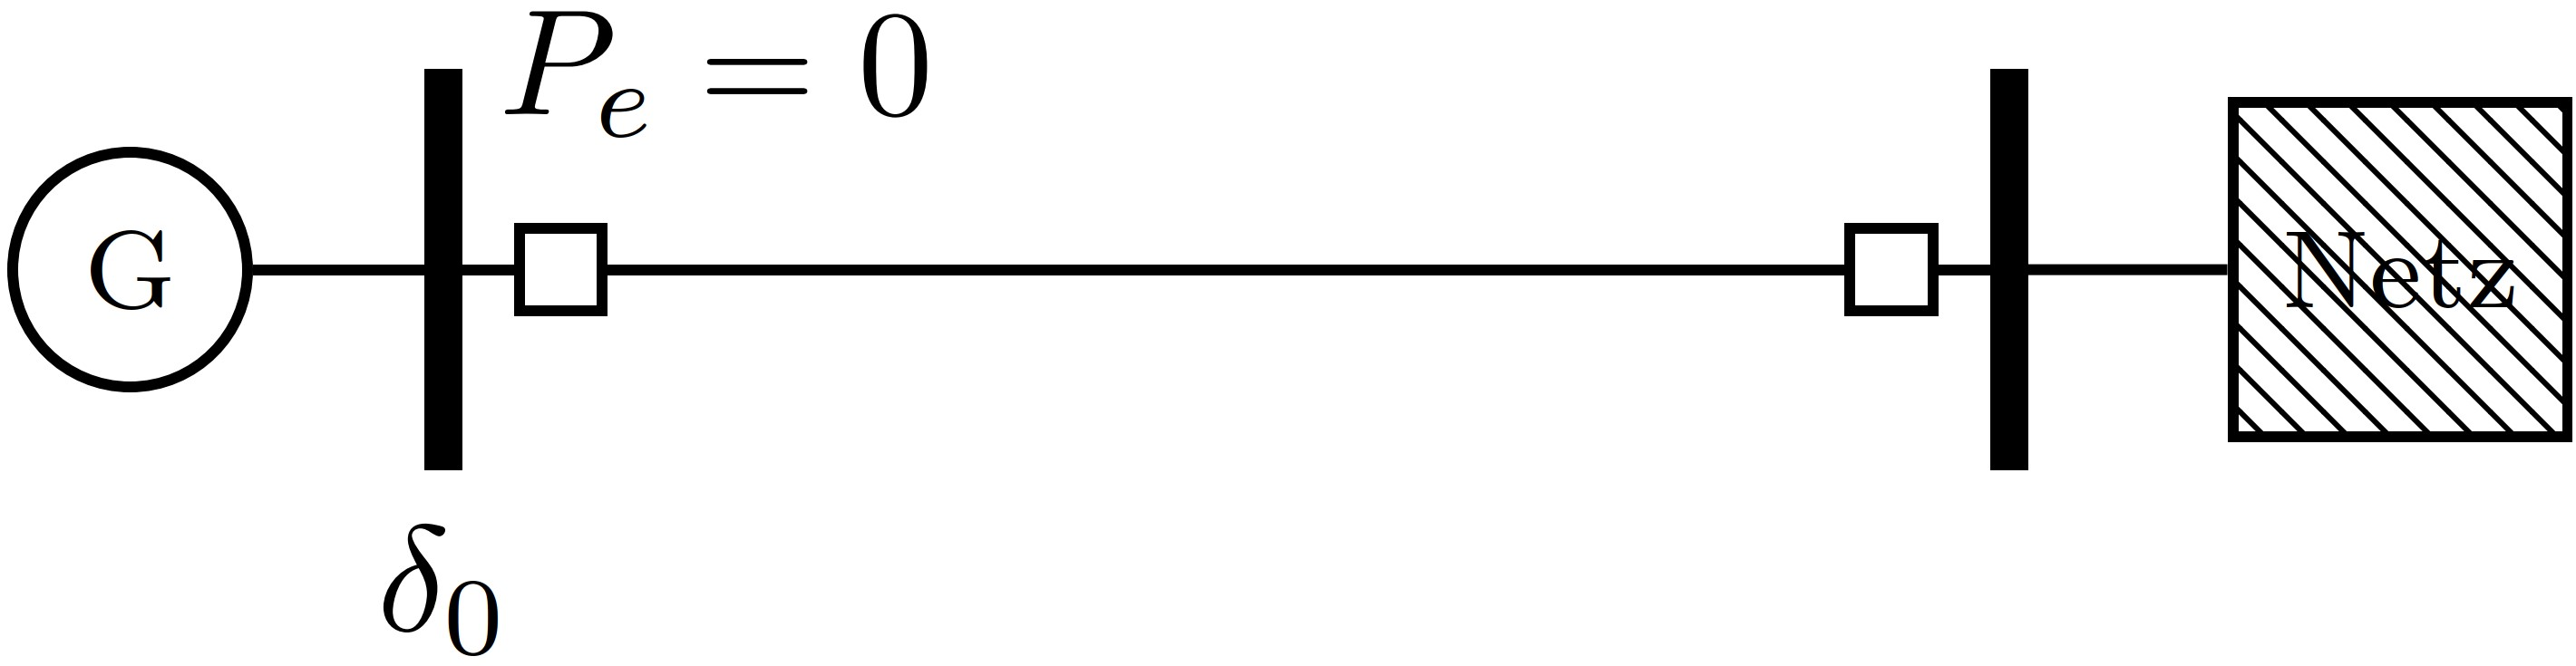
\includegraphics[width=0.95\linewidth]{images/Transiente_Stabilität_1.jpg}
    \end{minipage}%
    \hfill
    \begin{minipage}[t]{0.49\columnwidth}
        \centering \vspace{-0.7\baselineskip}
        $\boxed{\frac{d\omega}{dt} = \frac{P_m - P_{e}\big|_{=0}}{2H}}$
        $\quad$
        $\boxed{\frac{d\delta}{dt} = \omega}$
    \end{minipage}

    \vspace{0.1cm}

    \begin{minipage}[t]{0.35\columnwidth}
        \vspace{-0.3\baselineskip}
        Der Generator muss die von der Turbine zugeführte Energie $P_m$ aufnehmen, indem er seine kinetische Energie erhöht, d.h. beschleunigt:
        
        \vspace{0.1cm}
        
        $\frac{d\omega}{dt} > 0,\quad \omega \uparrow,\quad \delta \uparrow$
    \end{minipage}%
    \hfill
    \begin{minipage}[t]{0.59\columnwidth}
        \centering \vspace{-0.7\baselineskip}
        \renewcommand{\arraystretch}{1.2}
        \begin{tabular}{@{} l p{4cm} l @{}}
            $[\omega]$     & Winkelgeschwindigkeit \dotfill              & $\frac{\text{rad}}{\text{s}}$ \\
            $[t]$          & Zeit \dotfill                               & $\text{s}$ \\
            $[P_m]$        & mechanische Leistung \dotfill               & $\text{W}$ \\
            $[P_e]$        & elektrische Leistung \dotfill               & $\text{W}$ \\
            $[H]$          & Trägheitsfaktor \dotfill & - \\
            $[\delta]$     & Polradwinkel \dotfill                        & $\text{rad}$ \\
        \end{tabular}
    \end{minipage}

\subsubsection{Wiedereinschalten nach Fehlerfall}
    \begin{minipage}[t]{0.49\columnwidth}
        \centering \vspace{-0.7\baselineskip}
        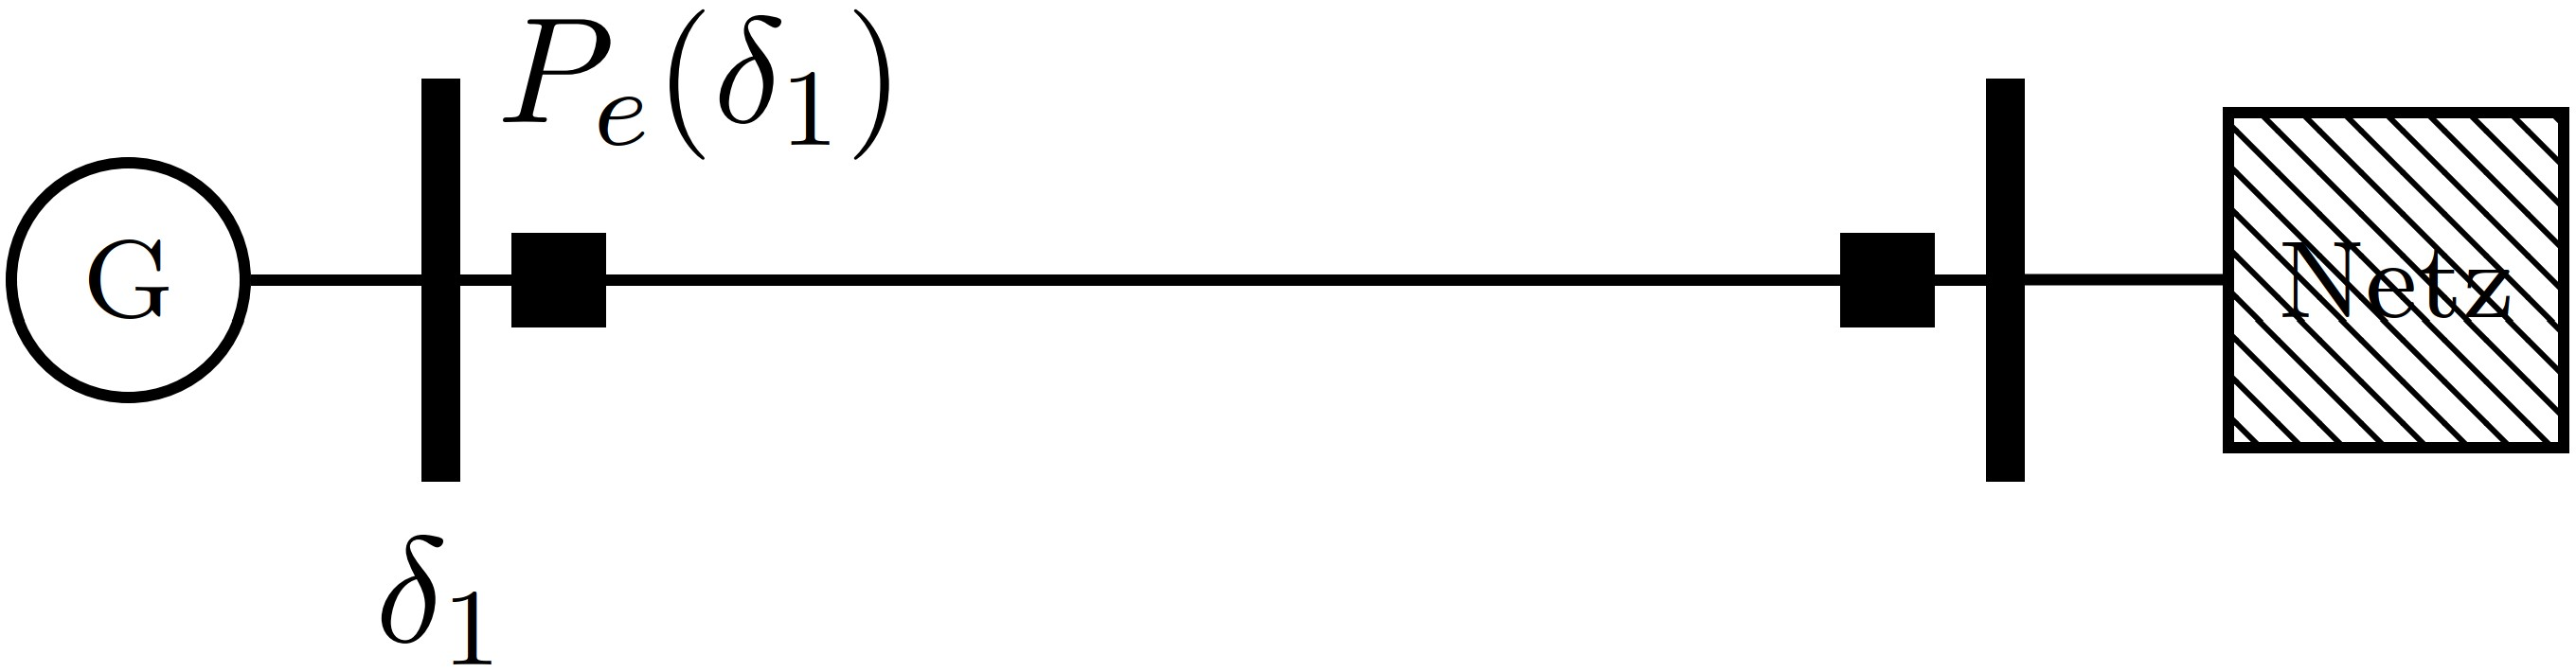
\includegraphics[width=0.95\linewidth]{images/Transiente_Stabilität_2.jpg}
    \end{minipage}%
    \hfill
    \begin{minipage}[t]{0.49\columnwidth}
        Nach wenigen Sekundenbruchteilen kommt es zu einer sogenannten automatischen Wiedereinschaltung: 
        In der Hoffnung, dass der Lichtbogen erloschen ist, schaltet das Schutzgerät die Leitung wieder zu. 
        
    \end{minipage}

    Die Schalter an beiden Leitungsenden werden nach Ablauf der Wiedereinschaltzeit (z.\,B. 500 ms) geschlossen.

    \vspace{0.1cm}

    In dieser Zeit ist $\delta$ gestiegen ($\delta = \delta_1$). Bei der Wiedereinschaltung ist $P_e(\delta_1) > P_m$. 

    Der Generator bremst und baut so die überschüssige kinetische Energie ab.

\subsection{Flächenkriterium}
\begin{minipage}[t]{0.45\columnwidth}
    \centering \vspace{-0.7\baselineskip}
    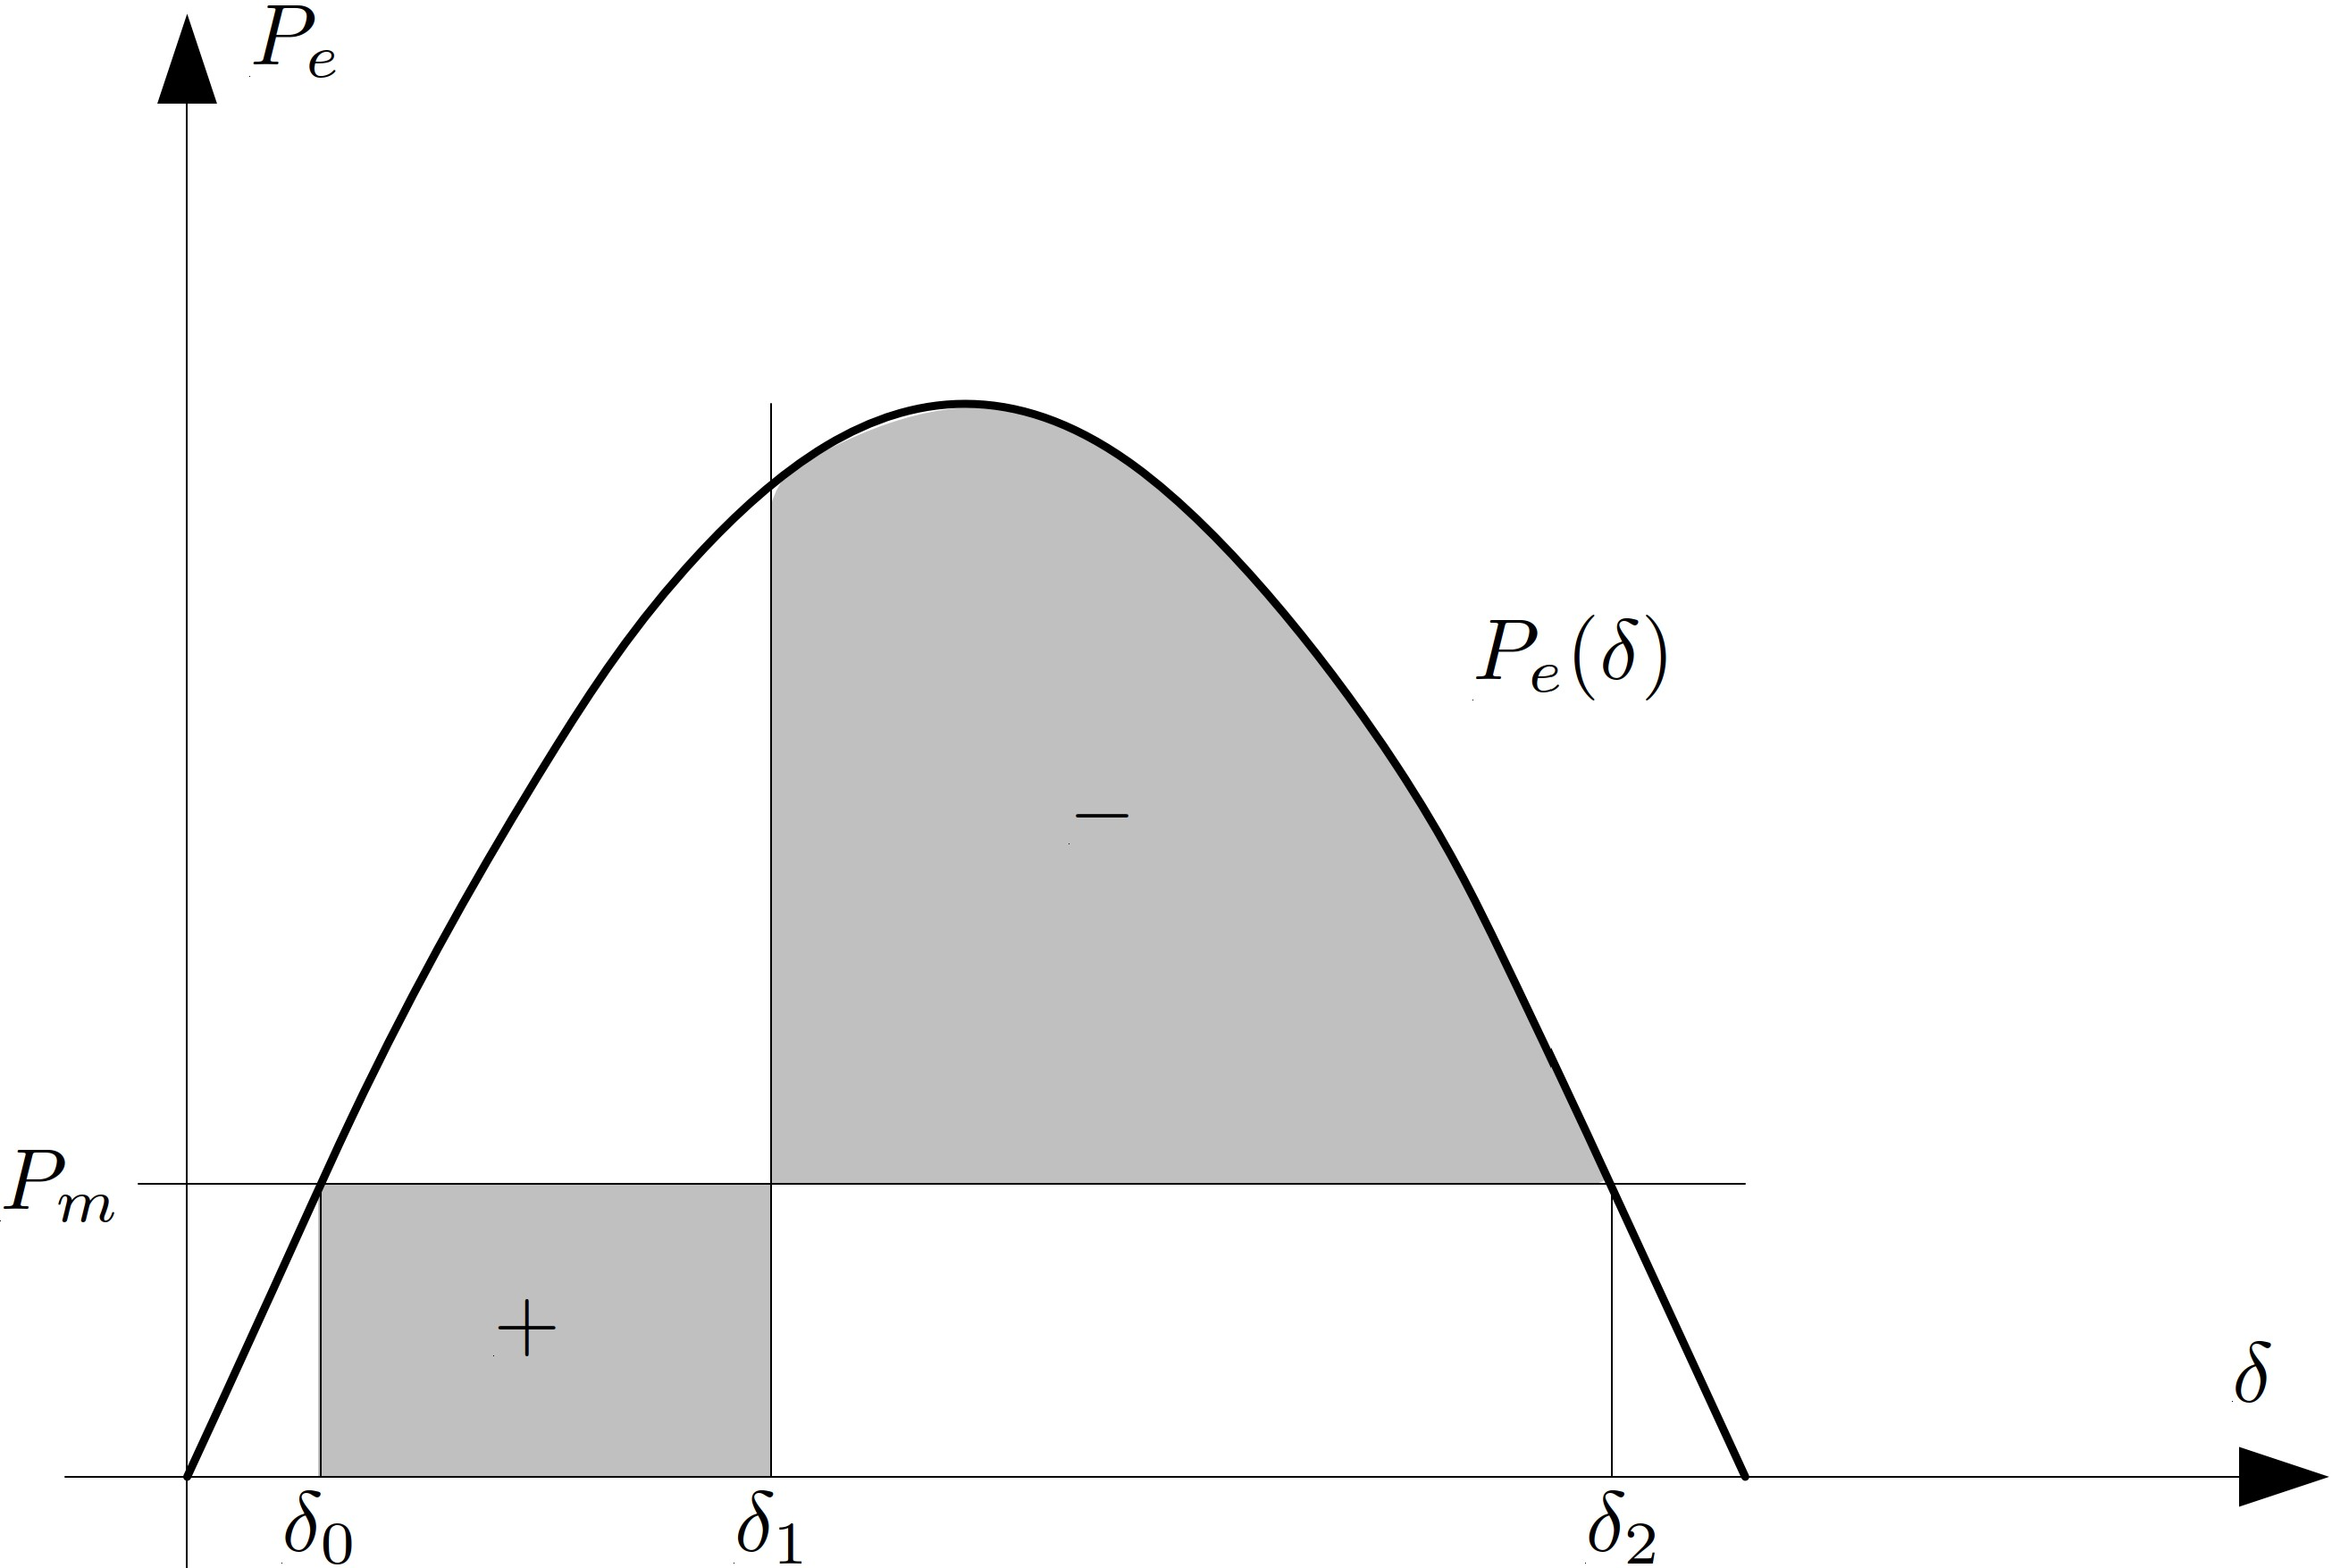
\includegraphics[width=0.85\linewidth]{images/Transiente_Stabilität_3.jpg}
\end{minipage}%
\hfill
\begin{minipage}[t]{0.54\columnwidth}
    \begin{itemize}
        \pro Fläche entspricht der Energie, die der Generator währen einer halben Sekunde aufnehmen muss
        \con Fläche entspricht der maximalen Energie, welche der Generator wieder abbauen kann
        \item Flächenkriterium: - Fläche muss grösser sein als + Fläche
        \item[]$\Rightarrow $\textbf{Flächenbeseitigungszeit} enorm wichtig
    \end{itemize}
\end{minipage}